% v11 RQ4: stress conditions, guards and scale (M2, M3, M5, M7, E2, E3, EX1, EX2, EX7, SM5).
\section{RQ4: Stress Conditions and Safety Guards}\label{sec:stress}
The controlled benchmark samples anchors that are long and unique enough to be found again, and its twelve edit types each receive equal weight. Its aggregate of \smCtlCasAccPct\% is therefore a score on a balanced benchmark of single, controlled transformations, not an estimate for naturally occurring revisions; on its four content-changing edit types alone the default reaches \ctlChangedAccPct\%. This section deliberately constructs harder conditions. Their rates describe the constructed cells and are not estimates of how often such cases occur; real-history prevalence is given by Section~\ref{sec:safety}. All stress inputs were generated, and the guards' code fixed, before evaluation on the held-out seed (protocol in the artifact).

\subsection{Indentation}
Normalization hides indentation (Section~\ref{sec:design}). To measure the consequence we constructed Python edits that preserve every normalized line but change nesting: a statement dedented out of its block, statements absorbed into the preceding block, one inner line of a multi-line anchor changing level, and a block moved one level with its header. Every generated file parses, and an edit counts as behaviour-changing when the abstract syntax tree of the enclosing scope changes. The deployed cascade requested no re-check for any of these: \bIndentMissDeployed{} of \bIndentSemanticN{} behaviour-changing edits kept their state. With the indentation guard none did (\bIndentMissIG{} of \bIndentSemanticN{}). The guard's cost appears on layout-only edits whose syntax tree is unchanged: it requested re-check for every continuation-line re-alignment (\bIndentFalseIG{} of \bIndentLayoutN{} layout-only edits overall).

The same experiment exposes a defect in the original benchmark. Its \emph{re-indent} operator, scored as an unchanged success, indents an anchor by four spaces without regard to syntax; of \BOriginalIndentTotalMain{} trials on the main seed, \BOriginalIndentInvalidMain{} produced files that no longer parse and \BOriginalIndentASTChangedMain{} produced parseable files with a changed syntax tree (replication: \BOriginalIndentInvalidReplication{} and \BOriginalIndentASTChangedReplication{} of \BOriginalIndentTotalReplication{}). Its \casReindent\% score measures normalized-text relocation, not safe handling of re-indented Python. We retain the original scores for comparability and report this qualification with them.

Real histories contain few such cases. Among all retained observations, \bRealIndentReturned{} returned spans match the old quotation after normalization but differ in indentation, and at the oracle's own locations \bRealIndentOracle{} do, all of them with unchanged statement trees. Indentation changes that alter behaviour are thus rare in the studied histories, and their real-history frequency, unlike their construction, is not established here.

\subsection{Duplicated, Short and Low-Information Anchors}
Supervisors often annotate short statements such as \texttt{return result}, an import or a repeated validation line. We constructed two stress suites. In the duplicate suite an identical copy of the anchored code is inserted near or far, above or below, or in another file, while the original is kept, edited, deleted or moved. In the short suite, one-line anchors are stratified by how often their normalized text recurs in the file and passed through the original edit types.

Duplicates are the cascade's weakest condition (Table~\ref{tab:duplicates}). The deployed cascade missed \bDupMissDeployed\% of the needed re-checks and placed \bDupSilentDeployed\% of the issues on the wrong code without a request; tier~2 chooses the copy nearest the old start, and a copy inserted just above the original occupies exactly that position. The pre-existing-copy guard reduced these to \bDupMissAG\% and \bDupSilentAG\%. It cannot help when the copy and the move are introduced in the same revision. One-line anchors fared better but still missed \bShortMissDeployed\% of needed re-checks, concentrated in the most frequently recurring lines. These results support a design change at annotation time as well as at relocation: when a supervisor anchors a line whose normalized text recurs in the file, the interface should ask for a longer selection.

\subsection{Guard Costs on Real Histories}
Each guard requests re-checks that the deployed cascade would not. Per 100 content-preserved real-history references, the indentation guard added \bIGExtraReal{} requests and the pre-existing-copy guard \bAGExtraReal{} at the default threshold, rising to \bIGExtraPubTgt{} and \bAGExtraPubTgt{} on public edit-targeted references; the variable-height window added none. On the \wpaMissTotal{} archived missed re-checks, the pre-existing-copy guard left \bArchivedMissAG{} unrequested and the combination of all three guards at $\theta=\wpaLopoTheta$ left \bArchivedMissAllCal{}. Because these cases motivated the guard, this is a mechanism check, not held-out evidence; the held-out evidence is the stress suites above and the external benchmark in Section~\ref{sec:external}.

\subsection{Variable-Height Windows}
Fixed-height windows cannot follow statements that grow or shrink (Section~\ref{sec:ranges}). With the variable-height window, public edit-targeted accuracy at the default threshold rose from \smPubTgtCasAccPct\% to \bVWPubTgtAcc\% and exact file/start/end recovery on surviving targets from \bRangeDeployedPubTgt\% to \bRangeVWPubTgt\%, with no additional re-check requests.

\subsection{Compound Edits}\label{sec:compound}
A resubmission rarely applies one transformation. We composed $k \in \{1,2,3,4\}$ distinct operators on the same anchor: a move within the file or to another file, an identifier rename inside the anchor, a layout-only wrap or re-alignment, an inserted or deleted inner statement, statements inserted directly above, and a token edit nearby. Lines carry construction tags, so the anchor's final location is known by construction, and an anchor counts as changed when the syntax trees of its statements differ. Every edited file parses. To keep moves and insertions parseable, anchors were restricted to complete runs of sibling statements; this and the rejection of inapplicable operator combinations make the cells a constructed stress test, not a sample of revisions. Each cell has 300 trials per seed on two seeds (\bTwoNOne{} per $k$ pooled; Table~\ref{tab:compound}, Fig.~\ref{fig:compound}).

% Generated by tools/v11/analyze_wpb2.py; do not edit.
\begin{table}[t]
\caption{Compound Edits: Both Seeds Pooled}\label{tab:compound}
\centering\footnotesize\setlength{\tabcolsep}{3pt}
\begin{tabular}{@{}rlrrrrr@{}}\toprule
$k$ & Method & Place & Range & Missed & Silent & Lost \\ \midrule
1 & Deployed cascade & 82.5 & 74.0 & 3.7 & 0.2 & 6.8 \\
 & All guards, $\theta=0.85$ & 96.5 & 94.7 & 0.0 & 0.0 & 2.0 \\
 & All guards, $\theta=0.55$ & 94.8 & 92.3 & 0.0 & 0.0 & 0.0 \\
 & Cascade v1 & 84.8 & 0.0 & 3.7 & 0.2 & 1.7 \\
 & Contextual tracker & 86.8 & 0.0 & 2.1 & 0.0 & 12.3 \\
 & Diff drift & 31.5 & 0.0 & 0.0 & 0.0 & 68.5 \\ \midrule
2 & Deployed cascade & 52.8 & 40.5 & 2.0 & 0.7 & 36.0 \\
 & All guards, $\theta=0.85$ & 68.5 & 65.8 & 0.0 & 0.0 & 27.5 \\
 & All guards, $\theta=0.55$ & 67.3 & 63.8 & 0.0 & 0.0 & 16.7 \\
 & Cascade v1 & 66.0 & 0.0 & 2.3 & 0.7 & 12.2 \\
 & Contextual tracker & 69.7 & 0.0 & 0.3 & 0.0 & 29.3 \\
 & Diff drift & 5.7 & 0.0 & 0.0 & 0.0 & 94.3 \\ \midrule
3 & Deployed cascade & 25.8 & 19.7 & 0.4 & 0.2 & 66.5 \\
 & All guards, $\theta=0.85$ & 35.8 & 34.3 & 0.0 & 0.0 & 61.2 \\
 & All guards, $\theta=0.55$ & 37.8 & 35.8 & 0.0 & 0.0 & 37.3 \\
 & Cascade v1 & 45.2 & 0.0 & 0.9 & 0.5 & 31.2 \\
 & Contextual tracker & 55.3 & 0.0 & 0.0 & 0.0 & 44.3 \\
 & Diff drift & 0.0 & 0.0 & 0.0 & 0.0 & 100.0 \\ \midrule
4 & Deployed cascade & 11.5 & 9.0 & 0.0 & 0.0 & 82.3 \\
 & All guards, $\theta=0.85$ & 18.0 & 17.3 & 0.0 & 0.0 & 78.5 \\
 & All guards, $\theta=0.55$ & 19.2 & 17.7 & 0.0 & 0.0 & 46.2 \\
 & Cascade v1 & 27.3 & 0.0 & 0.2 & 0.2 & 42.8 \\
 & Contextual tracker & 41.8 & 0.0 & 0.0 & 0.0 & 57.8 \\
 & Diff drift & 0.0 & 0.0 & 0.0 & 0.0 & 100.0 \\
\bottomrule
\end{tabular}
\tablenote{}{Percentages. Place: file and start among surviving targets. Range: exact file/start/end (blank for line-only methods, scored as incorrect). Missed: changed targets without a re-check request. Silent: wrong placement without a request.}
\end{table}


\begin{figure*}[t]
\centering
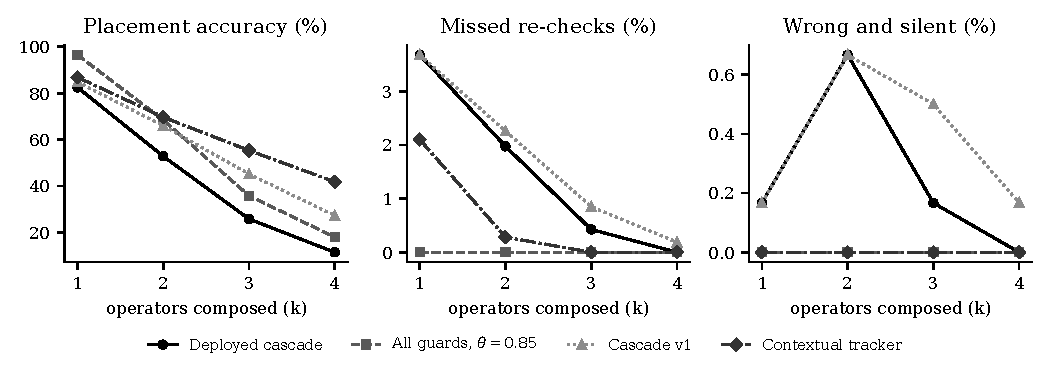
\includegraphics[width=\textwidth]{generated/compound-v11.pdf}
\caption{Compound edits: placement, missed re-checks and silent misplacement against the number of composed operators, both seeds pooled.}\label{fig:compound}
\end{figure*}

Placement accuracy of the deployed cascade fell from \bTwoDepAccOne\% for one operator to \bTwoDepAccTwo\%, \bTwoDepAccThree\% and \bTwoDepAccFour\% for two, three and four. The cascade failed by losing anchors, not by misplacing them: the lost share rose from \bTwoDepLostOne\% to \bTwoDepLostFour\%, while silent misplacement stayed at or below \bTwoDepSilentTwo\% and missed re-checks at or below \bTwoDepMissOne\%. A lost anchor returns its issue for re-check, so the composite failure is extra supervisor work rather than hidden error. The contextual tracker placed more starts from three operators on (\bTwoTrkAccThree\% and \bTwoTrkAccFour\%), but returns no range and never follows code into another file. The three guards together raised placement to \bTwoAllAccOne\%--\bTwoAllAccFour\% and range recovery to \bTwoAllRangeOne\%--\bTwoAllRangeFour\%, mainly through the variable-height window, at a large cost in requests on preserved code: \bTwoAllFalseOne\% of the single-operator preserved anchors were returned, against \bTwoDepFalseOne\% for the deployed cascade. Two causes dominate, and both concern the pre-existing-copy guard. By design it flags every move within a file, because a move does not increase the number of copies. It also flagged every pure insertion directly above an anchor: the pinned diff mapping places the expected start of an anchor whose preceding lines were inserted at the first inserted line, so the unmoved anchor never sits at its expected start. The insertion fix (AGi, Section~\ref{sec:guards}) removes this second cause. On a further compound seed generated after the fix was specified, AGi lowered the requests on single-operator preserved anchors from \wiFrCmpOneCasAGFalse\% to \wiFrCmpOneCasAGiFalse\% (all guards: \wiFrCmpOneCasGFalse\% to \wiFrCmpOneCasGiFalse\%) without a single additional missed re-check or silent misplacement. A stronger locator does not remove the decline with $k$: on the held-out seed alone (Table~\ref{tab:locator}; Table~\ref{tab:compound} pools both seeds), at four operators CodeMapper placed \wiFrCmpFourCmQPlace\% of the anchors and the contextual tracker \wiFrCmpFourTrQPlace\%, against \wiFrCmpFourDepPlace\% for the deployed cascade. Under every guarded locator, the compound failures were lost anchors, which return their issue, rather than silent ones (Section~\ref{sec:locator}).

\subsection{Multi-Anchor Issues}
The deployed rule returns an issue for re-check when any of its anchors changes or disappears. Its consequences grow with the number of anchors. We grouped $k$ distinct real-history anchors from the same commit pair into synthetic issues (\bTwoDistinctObs{} distinct observations; the first anchor is the primary). The grouping is synthetic: anchors from one commit pair need not belong to one concern. With one anchor, \bTwoIssueRecheckOne\% of issues were returned; with two, three, five, eight and twelve anchors, \bTwoIssueRecheckTwo\%, \bTwoIssueRecheckThree\%, \bTwoIssueRecheckFive\%, \bTwoIssueRecheckEight\% and \bTwoIssueRecheckTwelve\% were (\bTwoGroupsTwelve{} twelve-anchor groups from \bTwoGroupPairsTwelve{} commit pairs). With two anchors, \bTwoNonPrimaryTwo\% of the returned issues were returned only because of a supporting anchor, rising to \bTwoNonPrimaryEight\% with eight; a policy that watched the primary anchor alone would have missed \bTwoPrimaryMissTwo\% of the two-anchor issues whose code had changed and \bTwoPrimaryMissEight\% of the eight-anchor ones, against at most \bTwoAnyMissOne\% for the any-anchor rule. The any-anchor rule is therefore necessary for safety, but on many-anchor issues it returns nearly every issue after an edit-heavy revision. The interface should show which anchor triggered the request, as the studio's per-anchor notes already do, and supervisors should prefer few, precise anchors per issue.

\subsection{Repeated Resubmissions}\label{sec:prefixes}
Section~\ref{sec:chains} compared one direct relocation with ten successive ones only at the tenth commit. To see how errors accumulate, we re-ran the original syntax-tree reference from each chain's first commit to commits 1, 2, 3, 5 and 10, with the original exclusions; recomputed at commit 10 it reproduced every archived reference, and \bTwoChainEvery{} of the \bTwoDecidableTen{} targets were decidable at every prefix (Fig.~\ref{fig:chains}). The intermediate references are the same heuristic, not independent identity labels.

\begin{figure*}[t]
\centering
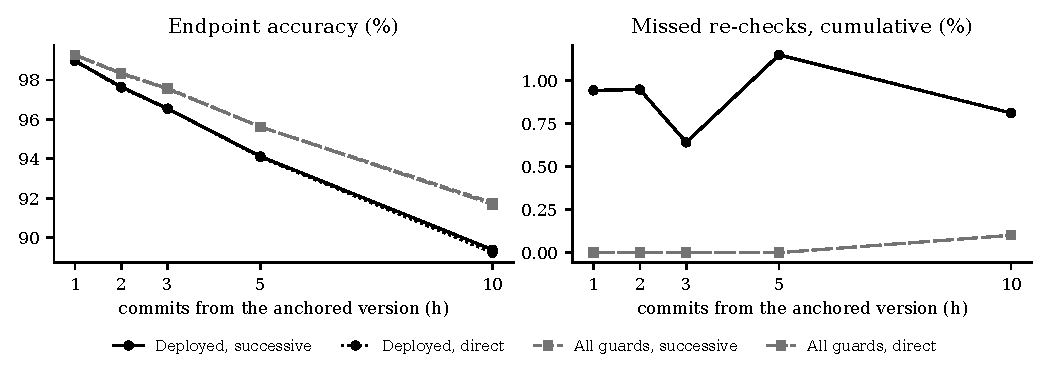
\includegraphics[width=\textwidth]{generated/chains-v11.pdf}
\caption{Accuracy and cumulative missed re-checks after $h$ commits, successive versus direct relocation, on the \bTwoChainEvery{} targets decidable at every prefix.}\label{fig:chains}
\end{figure*}

Successive and direct relocation stayed within a few tenths of a point of each other at every prefix. The figures in this paragraph are for the \bTwoChainEvery{} targets decidable at every prefix; Table~\ref{tab:identity} uses all \bTwoDecidableTen{} targets decidable at commit 10, so its counts differ slightly. Endpoint accuracy of the deployed cascade fell from \bTwoSeqAccOne\% after one commit to \bTwoSeqAccThree\%, \bTwoSeqAccFive\% and \bTwoSeqAccTen\% after three, five and ten, mostly through lost anchors (\bTwoSeqLostTen\% at ten commits) rather than wrong placements (\bTwoSeqWrongTen\%). Re-check requests persist in the issue's state, so the relevant safety measure is cumulative: of the \bTwoChangedTen{} targets whose code had changed by commit 10, \bTwoSeqMissTen\% had never been returned, and \bTwoSeqSilentTen\% of all targets sat on wrong code without any request. The last hop's label alone is a poor guide: a \lbl{changed} hop rewrites the stored quotation, so later hops compare against the rewritten text, and the final label failed to signal \bTwoSeqMissLastTen\% of the changes since the original. In \bTwoSeqLastExactWrongTen{} chains the endpoint was wrong while the last label read \lbl{identical} or \lbl{content-match}. The issue state, not the latest label, is what keeps such cases in front of the supervisor; once a supervisor clears a re-check, later labels describe change since the last cleared version only.

The calibrated threshold traded these failures differently. At $\theta=0.5$, accuracy after ten commits was \bTwoCalAccTen\%, but wrong placements reached \bTwoCalWrongTen\%, against \bTwoSeqWrongTen\% at the default, and \bTwoCalSilentLastTen\% of the targets sat on wrong code under a final label that requested nothing (\bTwoCalSilentTen\% had never been returned). Over repeated resubmissions the low threshold's misplacements accumulate, while the cumulative request history still catches nearly all of them. The three guards at the default threshold reduced cumulative missed re-checks to \bTwoSeqAllMissTen\% and silent misplacement to \bTwoSeqAllSilentTen\% after ten commits, with accuracy \bTwoSeqAllAccTen\%.

% Generated by tools/v11/build_wpi_tex.py from summary-20261102T183407.json; do not edit.
\begin{table}[t]
\caption{Ten Successive Commits: Identity Rule}\label{tab:identity}
\centering\footnotesize
\setlength{\tabcolsep}{2.4pt}
\begin{tabular}{@{}lrrrrrr@{}}\toprule
Method & \shortstack[r]{Correct} & \shortstack[r]{Wrong} & \shortstack[r]{Lost} & \shortstack[r]{Never\\returned} & \shortstack[r]{Last\\silent} & \shortstack[r]{Wrong,\\silent} \\ \midrule
Cascade & 89.4 & 2.2 & 8.4 & 8 & 563 & 85 \\
\quad + identity rule & 89.4 & 2.2 & 8.4 & 8 & 8 & 10 \\
Guarded, $\theta{=}0.55$ & 97.0 & 2.5 & 0.5 & 0 & 858 & 93 \\
\quad + identity rule & 97.0 & 2.5 & 0.5 & 0 & 3 & 4 \\
CodeMapper, labels & 97.7 & 2.0 & 0.3 & 3 & 865 & 71 \\
\quad + identity rule & 97.0 & 0.9 & 2.0 & 3 & 3 & 3 \\
CodeMapper, guarded & 97.7 & 2.0 & 0.3 & 0 & 865 & 71 \\
\quad + identity rule & 97.0 & 0.9 & 2.0 & 0 & 3 & 3 \\
CodeMapper, direct & 97.7 & 2.0 & 0.3 & 0 & 0 & 0 \\
\bottomrule
\end{tabular}
\tablenote{}{Endpoint after ten commits on 4,000 targets decidable at commit 10; correct, wrong and lost in \%. Never returned and last silent count, of the 989 targets whose code had changed since the first commit, those never returned at any hop and those not returned by the last hop's request; wrong, silent counts endpoints on wrong code with no request at the last hop. Guarded: the cascade with IG+AGi+VW; CodeMapper with IG+AGi (placement as labels only, by construction). CodeMapper is replayed hop by hop; direct maps the first version to the last, guarded, and is shown for reference.}
\end{table}


The identity rule (Section~\ref{sec:identity}, Table~\ref{tab:identity}) closes the gap between the last label and the history. Replayed over the same chains with the default cascade, it reduced the changes since the original that the tenth label failed to signal from \wiChIOffMissLastTenK{} to \wiChIOffIdMissLastTenK{}, the number never returned at any hop, and the endpoints on wrong code under a final label that requested nothing from \wiChIOffSilentLastTenK{} to \wiChIOffIdSilentLastTenK{}. The latest request now carries the history. With the recommended guards (IG+AGi+VW) at the calibrated threshold, the rule cut the unsignalled changes from \wiChICaliMissLastTenK{} to \wiChICaliIdMissLastTenK{} and the silent wrong endpoints from \wiChICaliSilentLastTenK{} to \wiChICaliIdSilentLastTenK{}; AG2 in place of AGi reached the same endpoints (\wiChICaltwoAccTen\% correct) but left \wiChICaltwoMissCumTenK{} change never returned, against \wiChICaliMissCumTenK{}. At the default floor of 0.5 the rule moved no cascade endpoint at either threshold, and a floor of 0.3 gave the same results. A floor of 0.7 left the default threshold unchanged but, at the calibrated one, turned changed hops less than 0.7 similar to the reviewed text into losses: correct endpoints \wiChICaliIdHighAccTen\% against \wiChICaliIdAccTen\%, wrong \wiChICaliIdHighWrongTen\% against \wiChICaliIdWrongTen\%, lost \wiChICaliIdHighLostTen\% against \wiChICaliIdLostTen\%. The rule matters for a stronger locator. CodeMapper replayed hop by hop placed \wiChICmSeqAccTen\% of the endpoints after ten commits, against \wiChIOffAccTen\% for the deployed cascade, with \wiChICmSeqWrongTen\% on wrong code; with the rule, wrong placements fell to \wiChICmSeqIdWrongTen\% and lost anchors rose from \wiChICmSeqLostTen\% to \wiChICmSeqIdLostTen\%, so uncertain transitions became visible losses instead of silent drift. With IG+AGi over CodeMapper, no change since review went unreturned at any hop (\wiChICmSeqGiMissCumTenK{}, against \wiChICmSeqMissCumTenK{} with labels only). The identity rule does not decide identity; it records which transitions were uncertain and keeps them in front of the supervisor.

Repeating CodeMapper on the same chains exposed a reproducibility limit. For the AGi replay every CodeMapper trace was recomputed, and \wiChIGateChains{} of the 4,000 chains differed from the first run (\wiChIGateMismatches{} traces or direct mappings); re-running those chains in one process returned different regions for identical inputs. The pinned CodeMapper is therefore not fully deterministic. The cascade reproduced exactly. All CodeMapper rows of Table~\ref{tab:identity} come from the second run, so its guarded and unguarded rows are paired.

\subsection{Scale}\label{sec:scale}
For an anchor of $s$ lines and $q$ characters in a file of $L$ lines, in a version of $N$ lines in total, the tiers cost: a digest comparison (tier~1); $O(L\,s)$ line comparisons for the exact run search (tier~2); a line diff of the old and new file, quadratic in $L$ in the worst case, plus $2r+1$ window comparisons with $r=\max(10,2s)$, each quadratic in $q$ in the worst case (tier~3); and $O(N\,s)$ for the cross-file search (tier~4). The pinned code recomputes the normalized lines of every file for each anchor that reaches tier~4, so a composition of $A$ such anchors costs $O(A\,N\,s)$; caching normalized files per composition would remove the factor $A$ from the file scan.

We timed composition on two large public trees, Django (\bTwoDjFiles{} files, \bTwoDjLines{} lines) and the CPython standard library (\bTwoPyFiles{} files, \bTwoPyLines{} lines), relocating 1,000 anchors sampled from files changed between consecutive releases (pinned commits in the artifact). The deployed cascade needed a median of \bTwoDjDepAnchorMed{}\,ms per anchor on Django and \bTwoPyDepAnchorMed{}\,ms on CPython (95th percentiles \bTwoDjDepAnchorPninetyfive{} and \bTwoPyDepAnchorPninetyfive{}\,ms), and \bTwoDjDepComposeThousand{}\,s and \bTwoPyDepComposeThousand{}\,s for the 1,000-anchor composition. Anchors found nowhere dominate: on CPython the \bTwoPyRemovedCount{} anchors labelled \lbl{removed} took \bTwoPyRemovedShare\% of the composition time. The adversarial case, a quotation found nowhere, forces the full cross-file scan and took a median of \bTwoDjDepAbsentMed{}\,ms per anchor on Django and \bTwoPyDepAbsentMed{}\,ms on CPython. The research implementation of the three guards is not optimized (median \bTwoDjAllAnchorMed{} and \bTwoPyAllAnchorMed{}\,ms per anchor). Timings come from one workstation and are descriptive; a capstone submission is far smaller than either tree.
